\documentclass{article}
\usepackage{amsmath}
\usepackage{graphicx}
\title{Catalina 1 Analytic vs. Numerical Solution}

\begin{document}

\maketitle

\section{Problem}

Compute the analytic and numerical solutions of the following shallow water problem:

\[
\begin{aligned}
\eta = e^{-(x-5)^2} \\
u = 0 \\
h = x \\
m = \infty  \\
\end{aligned}
\]

In other words, a Gaussian initial wave with 0 initial velocity, and a plane.

\section{Setup}

\subsection{Numerical}

We modified Deny's Catalina 1 finite volume to build 

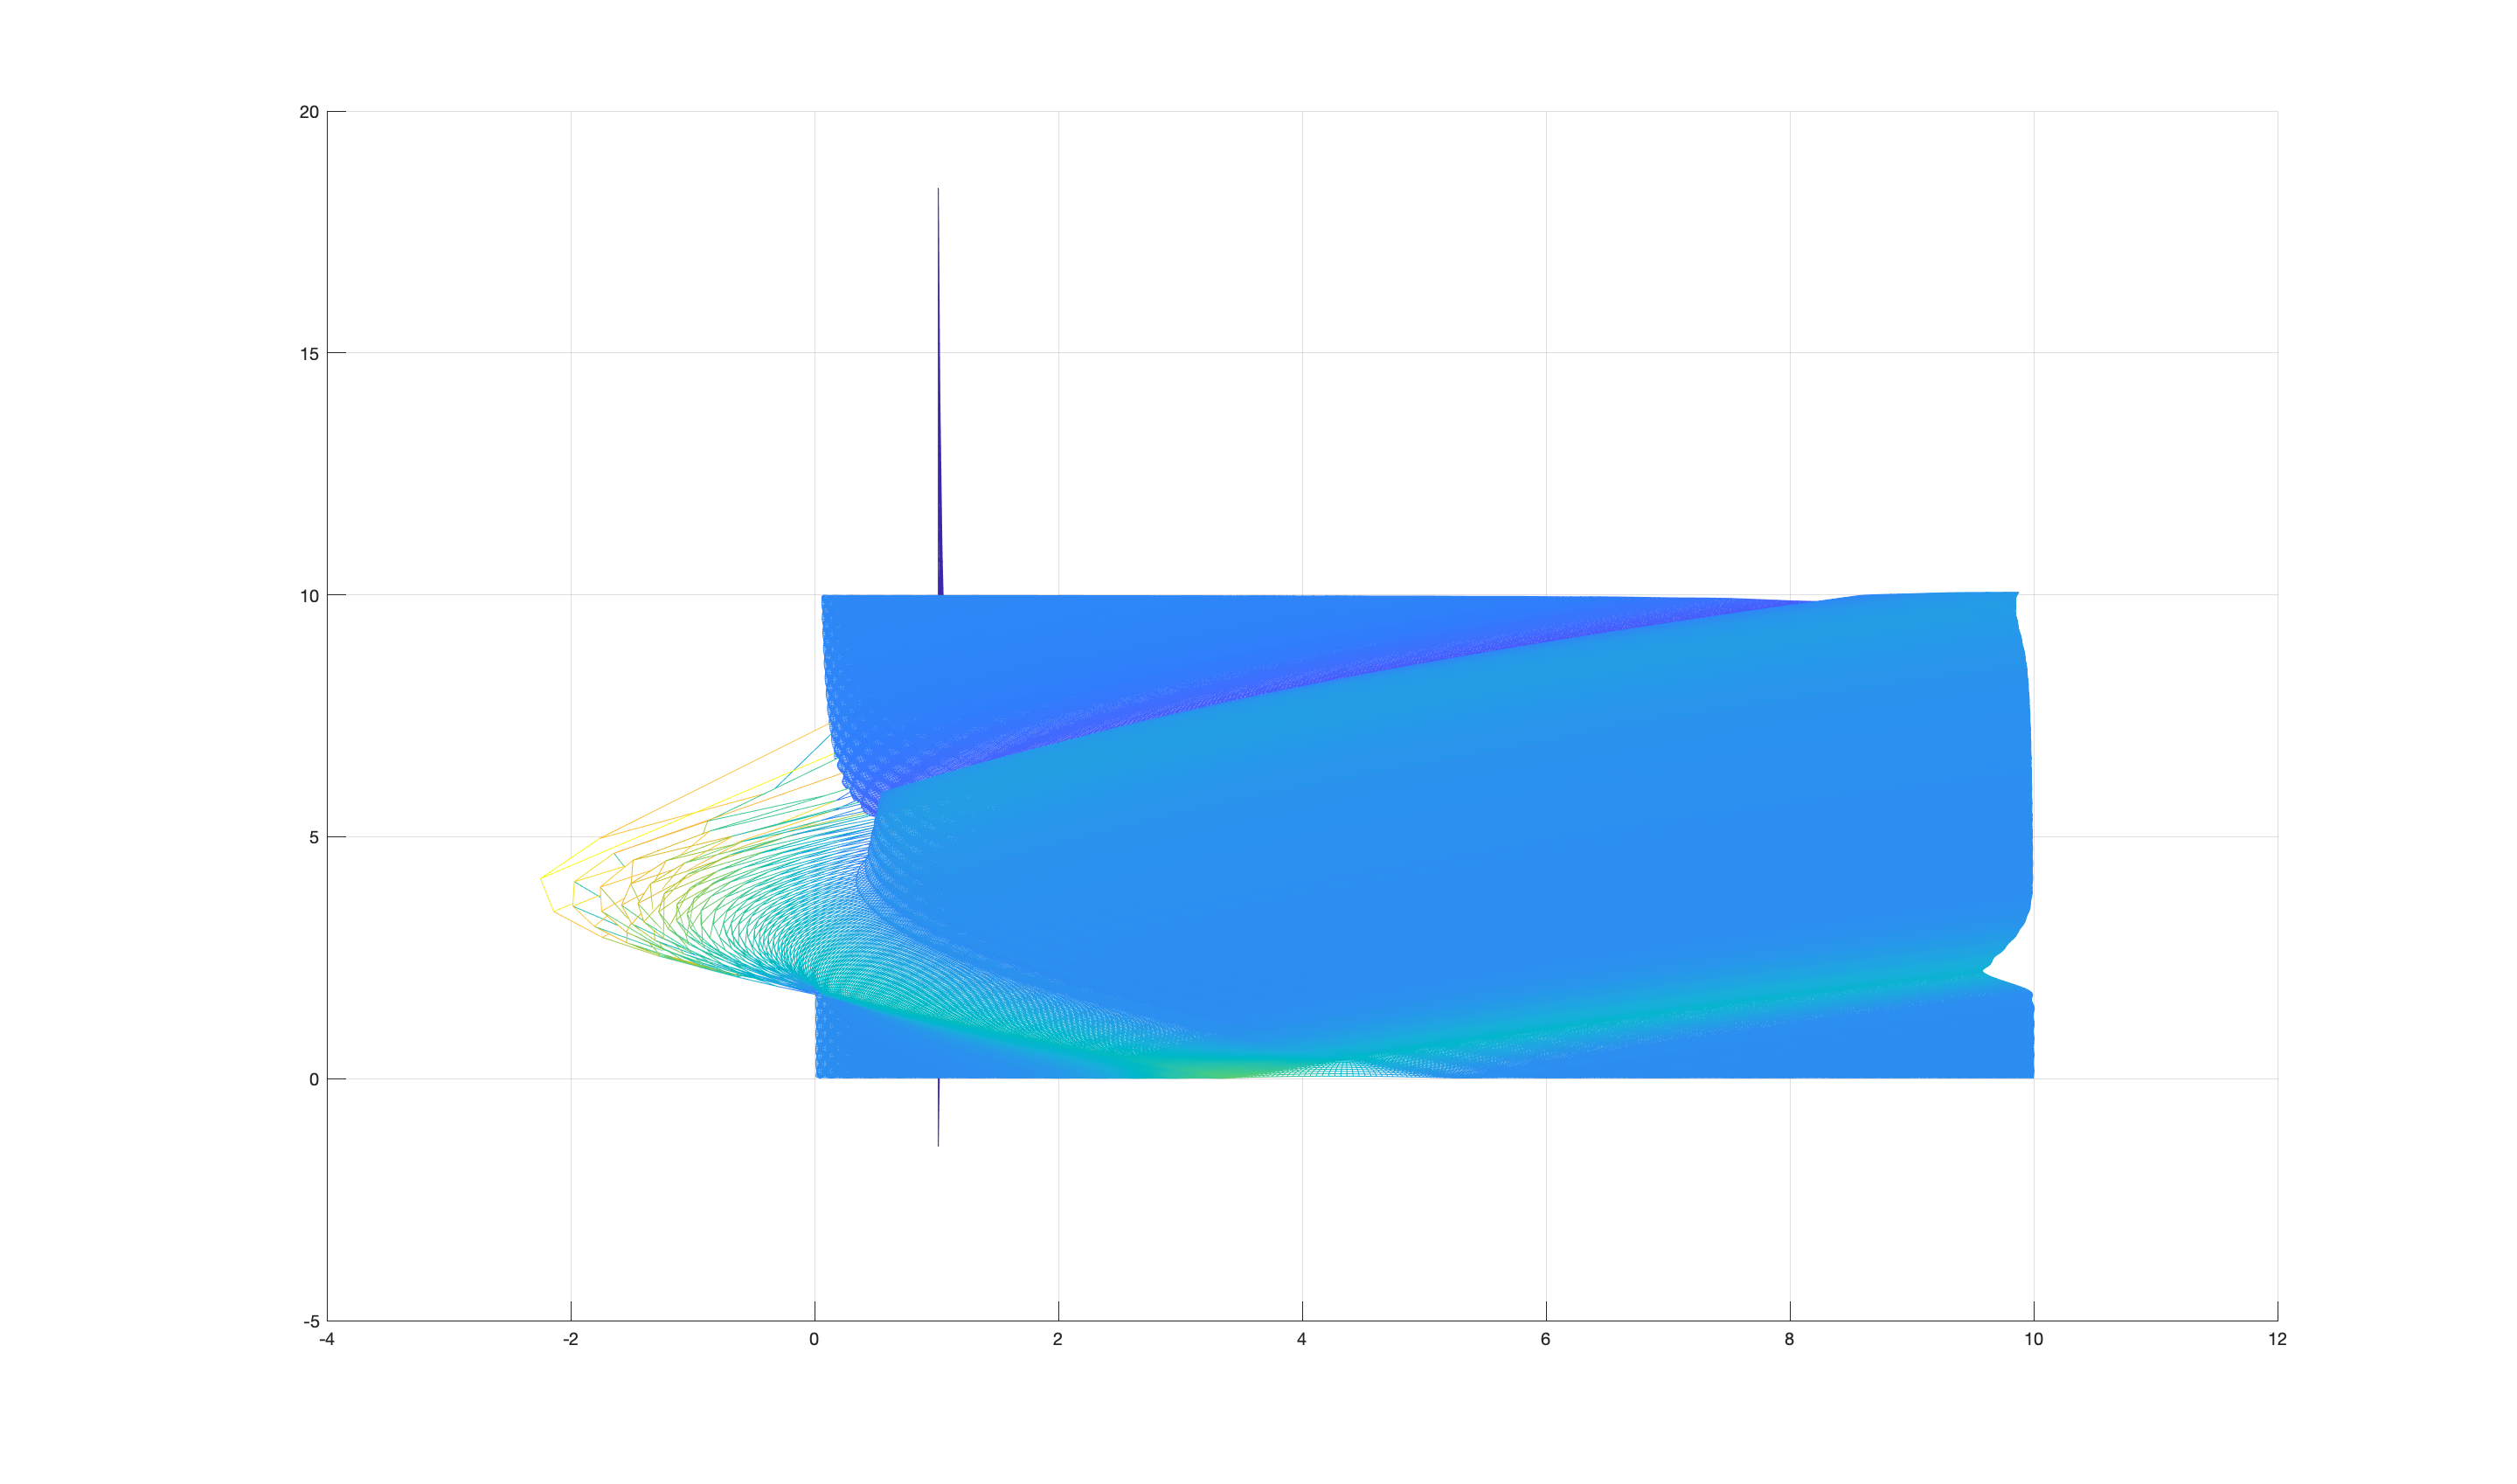
\includegraphics[width=\linewidth]{images/anaylytic.png}

\subsection{Anaylytic}

We used Chebfun to calculate the Hankel transform solution to the SWE. We 

\section{Statistical Analysis}

We used an L2 norm

\section{Further Problems}

Comparison of the computation of U


\end{document}
